\setcounter{figure}{0}
\setcounter{table}{0}
\setcounter{page}{1}
\renewcommand{\thefigure}{S\arabic{figure}}
\renewcommand{\thetable}{S\arabic{table}}
\renewcommand{\thepage}{S\arabic{page}}
  
%%% TITLE %%%
\title{\Large \bf Supplementary Information: Canalization of the evolutionary trajectory of the human influenza virus}
\maketitle

\section*{Supplementary discussion}

\subsection*{Punctuated antigenic change}

Antigenically similar phenotypes cluster together (Fig.~\ref{incmaptree}B) and antigenic clusters replace one another through time (Fig.~\ref{phenotypes}B).  Across replicate simulations, these clusters persist for an average of 5.0 years (interquartile range of 3.7--6.1 years) measured as the time it takes for a new cluster to reach 10\% frequency, peak and decline to 10\% frequency.  The transition between clusters occurs quickly, taking an average of 1.8 years (interquartile range of 1.1--2.3 years).   Antigenic evolution occurs in a punctuated fashion; periods of relative stasis are interspersed with more rapid antigenic change (Fig.~\ref{phenotypes}C).  Large discontinuities in antigenic phenotype frequently correspond to cluster transition events.  Over the  40-year simulation, antigenic drift moves the virus population at an average rate across replicates of 1.05 antigenic units per year (interquartile range 0.96--1.14). 

Antigenic and epidemiological dynamics show a fundamental linkage, so that large jumps of antigenic phenotype result in increased rates of infection (Fig.~\ref{incmaptree}A and B).  We observe a general correlation between year-to-year antigenic drift and attack rates the following year (corr = 0.27, Fig.~\ref{driftvsinc}A).  Similar patterns have been noted in influenza H3N2 in correlating excess mortality and antigenic evolution \cite{Wu10}.  Additionally, as noted by Koelle et al.\cite{Koelle06}, we commonly observe refractory years after a year of severe incidence brought about by antigenic drift (Fig.~\ref{incmaptree}A).  In general, years with low attack rates follow both unusually severe and unusually mild years (Fig.~\ref{driftvsinc}B).  

Yearly attack rates show significant variation, with an interquartile range across replicates of 0.9\% to 10.9\% in temperate regions and 2.8\% to 10.2\% in the tropics (Fig.~\ref{incmaptree}A).  When antigenic phenotype remains static, there may be multiple consecutive seasons without appreciable incidence, a pattern apparently absent from H3N2 influenza \cite{Finkelman07}.  We suggest that any model exhibiting punctuated evolution broadly consistent with the punctuated change seen in the antigenic map will show similarly varying patterns of incidence.  We can `fix' the incidence patterns, but at the cost of too smooth an antigenic map (Fig.~\ref{incmaptree_smooth}).  Evolutionary patterns of the neuraminidase (NA) protein may provide an explanation.  Epitopes in the HA and NA proteins are jointly responsible for determining antigenicity \cite{Nelson07NatRevGenet}, and it is now clear that levels of adaptive evolution are similar between HA and NA \cite{Bhatt11}.  Thus, changes in NA may be driving incidence patterns as well, resulting in an observed timeseries of incidence partially divorced from the antigenic map of HA.

\subsection*{Short-lived strain-transcending immunity}

It remains a central question as to the extent that short-lived strain-transcending immunity is responsible for influenza's limited diversity and spindly genealogical tree \cite{Ferguson03,Tria05}.  Our findings suggest a possible resolution.  Although lacking short-lived immunity, our model shows a detailed correspondence to both the antigenic map and genealogical tree of H3N2 influenza.  If an antigenic map were to show a deep bifurcation, where two viral lineages move in different antigenic directions, then we would expect the same bifurcation to be evident in the genealogical tree.  Short-lived strain-transcending immunity provides a mechanism by which lineages may diverge in antigenic phenotype, but still interfere with one another.  This mechanism would explain a situation where bifurcations emerge in the antigenic map, but competition results in the extinctions of divergent antigenic lineages.  The empirical antigenic map \cite{Smith04} suggests that this is not the case; one cluster leads to another cluster in orderly succession and there is never competition between two antigenically novel clusters.  This supports the hypothesis that antigenic evolution is primarily limited by a lack of mutational input.  This is not to say that short-lived strain-transcending immunity is not present; observed interference between subtypes \cite{Ferguson03,Goldstein11} provides substantial evidence for its existence.  Instead, we suggest that short-lived strain-transcending immunity does not automatically generate antigenic maps and genealogical trees consistent with empirical evidence.

%%% REFERENCES %%%
\bibliographystyle{plos2009}
\bibliography{/Users/bedfordt/Documents/bedford}

\vspace{1cm}

\section*{Supplementary Tables and Figures}

%%% Table S1: mktable %%%
\begin{table}[h]
	\centering
	\caption{\textbf{Rates of mutation and phenotypic change on trunk and side branches and mutational expectation.}}
	\label{mktable}
	\begin{tabular}{ l c c c c } 
	\hline
		 								& Baseline 	& Side branch 	& Trunk		& Trunk / side branch \\
	\hline				
	Mutation size (AG units)			& 0.60		& 0.79			& 1.58		& 1.99$\times$ \\
	Mutation rate (mut per year)		& 0.04		& 0.06			& 0.81		& 13.23$\times$ \\	
	Antigenic flux (AG units per year)	& 0.02		& 0.05			& 1.27		& 26.25$\times$ \\		
	\hline
	\end{tabular}
\end{table}

\pagebreak

%%% Figure S1: phenotypes %%%
\begin{figure}[H]
	\centering
	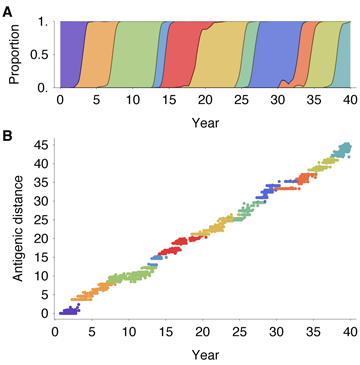
\includegraphics{figures/phenotypes}
	\caption{\textbf{Antigenic evolution over the course of the 40-year simulation}. (A) Two-dimensional antigenic phenotypes of 5943 viruses.  Each discrete virus phenotype is shown as a bubble, with bubble area proportional to the number of times this phenotype was sampled. (B) Proportion of virus population comprised of each antigenic cluster through time.  (C) Antigenic distance from initial phenotype ($x=0,y=0$) for each of 5943 virus samples relative to time of virus sampling. In (A) and (C) viruses were sampled at a constant rate proportional to prevalence and coloring was determined by clustering samples on the antigenic map in figure \ref{incmaptree}B.}
	\label{phenotypes}
\end{figure}

\pagebreak

%%% Figure S2: incdrift %%%
\begin{figure}[!c]
	\centering
	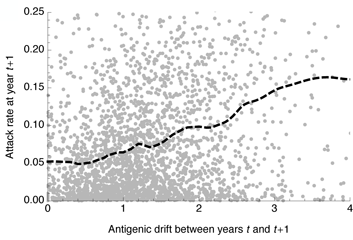
\includegraphics{figures/driftvsinc}
	\caption{\textbf{Correlation between antigenic drift and incidence and autocorrelation of attack rate}. (A) Antigenic drift measured as the distance between the centroid of phenotypes at year $t$ and the centroid of phenotypes at year $t+1$ vs.\ incidence measured as the number of samples out of $\sim6000$ in each replicate simulation taken at year $t+1$. (B) Temperate attack rate at year $t$ vs.\ temperate attack rate at year $t+1$. In both cases, individual pairs of measurements are shown as gray points and a locally-linear regression (LOESS) as black dashed line.}
	\label{driftvsinc}
\end{figure}

\pagebreak

%%% Figure S2: mutspectrum %%%
\begin{figure}[!c]
	\centering
	\makebox[\textwidth]{		
		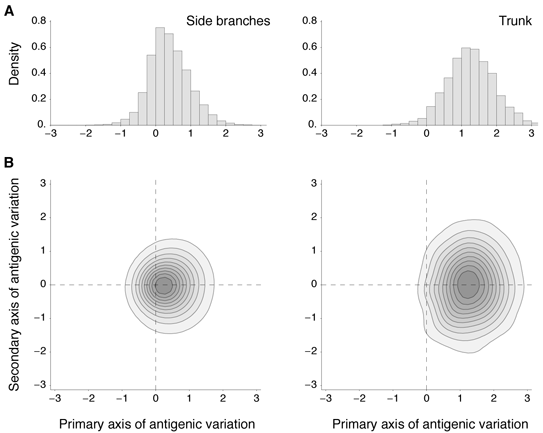
\includegraphics{figures/mutspectrum}
	}
	\caption{\textbf{Mutation spectrum in two-dimensional antigenic space of side branch mutations and trunk mutations}. (A) Smoothed histogram of mutation effects along the axis of primary antigenic variation across 80 replicate simulations.  Left panel shows the distribution of effects of side branch mutations and the right panel shows the distribution of effects of trunk mutations. (B) Smoothed two-dimensional histogram of mutation effects along the primary and secondary axes of antigenic variation across 80 replicate simulations.  Histograms were constructed from 21,405 side branch mutations and 1584 trunk mutations.}
	\label{mutspectrum}
\end{figure}

\pagebreak

%%% Figure S3: probtrunk %%%
\begin{figure}[!c]
	\centering
	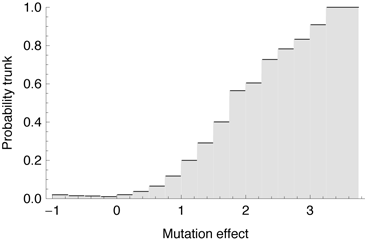
\includegraphics{figures/probtrunk}
	\caption{\textbf{Relationship between a mutation's phenotypic effect and its likelihood of being part of the trunk}. The $x$-axis represents the effect of a mutation along the line of primary antigenic variation, and the $y$-axis represents the probability that the mutation is part of the trunk.  Mutations of large effect are increasingly rare, but when they do occur are increasingly likely to be part of the trunk.}
	\label{probtrunk}
\end{figure}

\pagebreak

%%% Figure S5: waittimes %%%
\begin{figure}[!c]
	\centering
	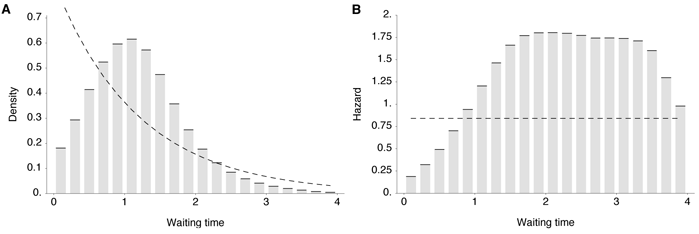
\includegraphics{figures/waittimes}
	\caption{\textbf{Observed vs.\ expected distributions of waiting times between phenotypic mutations along genealogy trunk.} (A) Histogram bins show the observed distribution of waiting times in years across 80 replicate simulations representing 1584 mutations.  The mean of this distribution is 1.76 years.  The dashed line shows the Poisson process expectation of exponentially distributed waiting times.  (B) The discrete distribution of waiting times is transformed into a discrete hazard function, representing the rate of trunk mutation after a specific waiting time.  The dashed line shows the memoryless hazard function of the Poisson process expectation.}
	\label{waittimes}
\end{figure}

\pagebreak

%%% Figure S8: h1n1_mut %%%
\begin{figure}[!c]
	\centering
	\makebox[\textwidth]{
		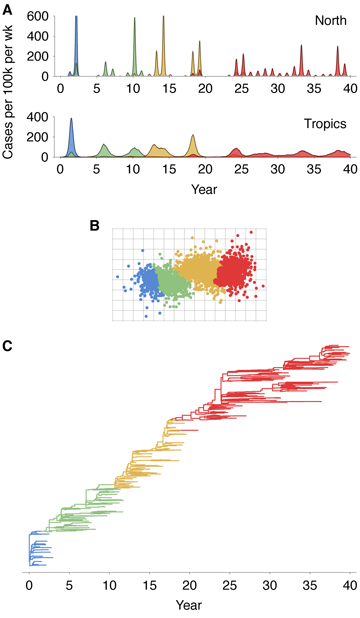
\includegraphics{figures/h1n1_mut}
	}
	\caption{\textbf{Simulation results showing epidemiological, antigenic and genealogical dynamics for weaker mutation model}. (A) Weekly timeseries of incidence of viral infection in north and tropics regions. (B) Antigenic map depicting phenotypes of viruses sampled over the course of the simulation.  Grid lines show single units of antigenic distance. (C) Genealogical tree depicting the infection history of samples from the virus population.  Cluster assignments were used to color panels (A), (B) and (C) in a consistent fashion.  Alternative mutational parameters are $\mu = 5 \times 10^{-5}$, mean mutation size of 0.42 units and standard deviation of mutation size of 0.28 units.}
	\label{h1n1_mut}
\end{figure}

\pagebreak

%%% Figure S8: h1n1_r0 %%%
\begin{figure}[!c]
	\centering
	\makebox[\textwidth]{
		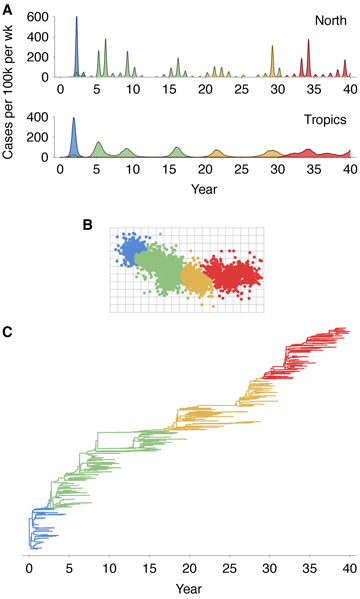
\includegraphics{figures/h1n1_r0}
	}
	\caption{\textbf{Simulation results showing epidemiological, antigenic and genealogical dynamics for lower instrinsic $R_0$}. (A) Weekly timeseries of incidence of viral infection in north and tropics regions. (B) Antigenic map depicting phenotypes of viruses sampled over the course of the simulation.  Grid lines show single units of antigenic distance. (C) Genealogical tree depicting the infection history of samples from the virus population.  Cluster assignments were used to color panels (A), (B) and (C) in a consistent fashion.  Alternative epidemiological parameters are $\beta = 0.3$ giving $R_0 = 1.5$.}
	\label{h1n1_r0}
\end{figure}

\pagebreak

%%% Figure S4: 10dgrid %%%
\begin{figure}[!c]
	\centering
	\makebox[\textwidth]{	
		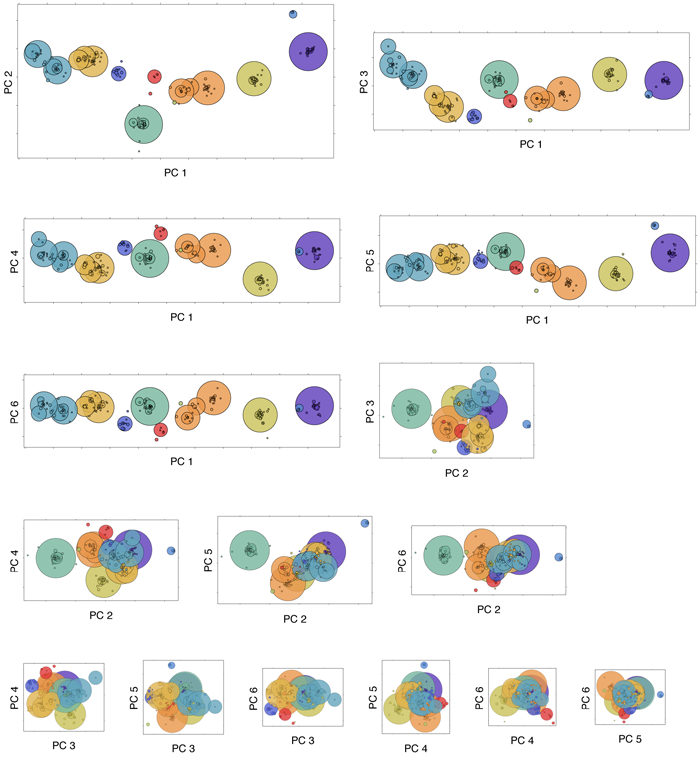
\includegraphics{figures/10dgrid}
	}
	\caption{\textbf{Principal components of antigenic variation under a 10-sphere mutation model}. Each panel shows approximately 6000 samples of antigenic phenotype over the course of a 40-year simulation.  Each phenotype is represented as a bubble, with bubble area proportional to the number of samples with this phenotype.  Bubbles are colored based on clustering the 10-dimensional antigenic phenotypes.  The original 10-dimensional space was rotated using principal components analysis to give orthogonal axes in the order of their contribution to antigenic variation.  Each panel shows a two-dimensional slice of the this rotated space.  Axes are consistent across panels.  Principal components 7--10 were left out of the figure for clarity.}
	\label{10dgrid}
\end{figure}

\pagebreak

%%% Figure 6: replicateevolfull %%%
\begin{figure}[!c]
	\centering
	\makebox[\textwidth]{	
		\includegraphics{figures/replicateevolfull}
	}
	\caption{\textbf{Antigenic phenotypes over the course of 5 years of evolution across 100 replicate simulations starting from identical initial conditions}.  Replicate simulations were initialized with the end state of the original 40-year simulation shown in figure \ref{incmaptree}.  The top left panel shows every antigenic phenotype present in the initial virus population.  The black point represents the population mean.  Each subsequent panel shows an additional year of evolution, with black points representing the mean antigenic phenotypes of the 100 replicate simulations and gray lines representing the history of each mean antigenic phenotype.}
	\label{replicateevolfull}
\end{figure}

\pagebreak

%%% Figure S6: replicatetimeseries %%%
\begin{figure}[!c]
	\centering
	\makebox[\textwidth]{
		\includegraphics{figures/replicatetimeseries}
	}
	\caption{\textbf{Timeseries of incidence across 100 replicate simulations with identical initial conditions.} Panels show incidence in the North, Tropics and South regions over the course of 10 years.  Solid black lines represent the median weekly incidence across the 100 replicate simulations, while gray intervals represent the interquartile range across simulations.  There is little variability for the first year of replicate simulations.  Replicate simulations were initialized with the end state of the original 40-year simulation shown in figure \ref{incmaptree}.}
	\label{replicatetimeseries}
\end{figure}

\pagebreak

%%% Figure S7: incmaptree_smooth %%%
\begin{figure}[!c]
	\centering
	\makebox[\textwidth]{
		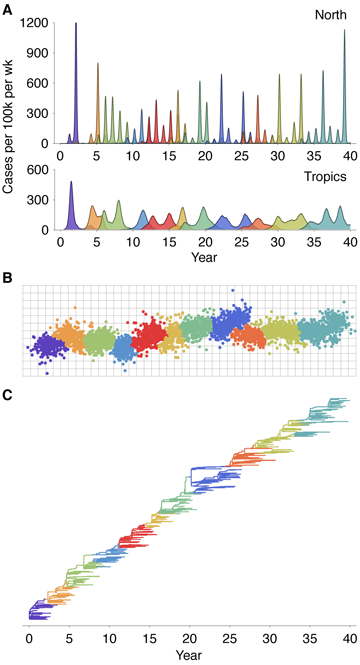
\includegraphics{figures/incmaptree_smooth}
	}
	\caption{\textbf{Simulation results showing epidemiological, antigenic and genealogical dynamics for `smoother' mutation model}. (A) Weekly timeseries of incidence of viral infection in north and tropics regions. (B) Antigenic map depicting phenotypes of viruses sampled over the course of the simulation.  Grid lines show single units of antigenic distance. (C) Genealogical tree depicting the infection history of samples from the virus population.  Cluster assignments were used to color panels (A), (B) and (C) in a consistent fashion.  Alternative mutational parameters are $\mu = 3 \times 10^{-4}$, mean mutation size of 0.6 units and standard deviation of mutation size of 0.2 units.}
	\label{incmaptree_smooth}
\end{figure}

\pagebreak

%%% Figure S8: incmaptree_rough %%%
\begin{figure}[!c]
	\centering
	\makebox[\textwidth]{
		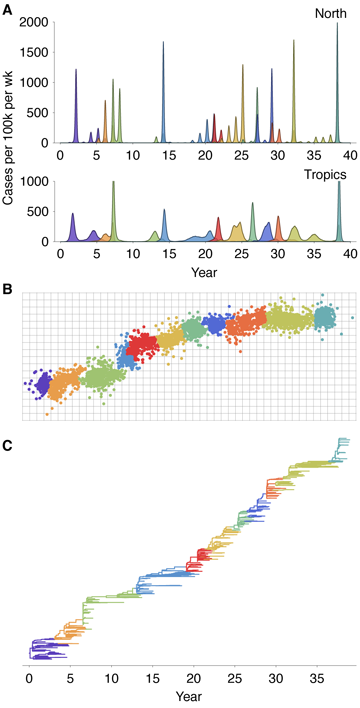
\includegraphics{figures/incmaptree_rough}
	}
	\caption{\textbf{Simulation results showing epidemiological, antigenic and genealogical dynamics for `rougher' mutation model}. (A) Weekly timeseries of incidence of viral infection in north and tropics regions. (B) Antigenic map depicting phenotypes of viruses sampled over the course of the simulation.  Grid lines show single units of antigenic distance. (C) Genealogical tree depicting the infection history of samples from the virus population.  Cluster assignments were used to color panels (A), (B) and (C) in a consistent fashion.  Alternative mutational parameters are $\mu = 5 \times 10^{-5}$, mean mutation size of 0.7 units and standard deviation of mutation size of 0.5 units.}
	\label{incmaptree_rough}
\end{figure}
